\chapter{Standards and Impacts} \label{Impact}
\ifpdf
    \graphicspath{{chapter_4/figures/PNG/}{chapter_4/figures/PDF/}{chapter_4/figures/}}
\else
    \graphicspath{{chapter_4/figures/EPS/}{chapter_4/figures/}}
\fi
%Write few lines about this chapter.

%\chapter{Impact}
%Write in details about the datasets that you used in this research work.%

%\begin{table}[htbp]
%\caption[Dataset]{Number of instances in dataset.}
%\centering
%\footnotesize
%\begin{tabular}{|c|c|c|} \hline
%\bf Attack Types & \bf Training Examples & \bf Testing Examples \\\hline
%Normal & 97278 & 60592 \\\hline
%Denial of Service & 391458 & 237594 \\\hline
%Remote to User & 1126 & 8606 \\\hline
%User to Root & 52 & 70 \\\hline
%%Probing & 4107 & 4166 \\\hline
%Total Examples & 494021 & 311028 \\\hline
%\end{tabular}
%\label{training_testing_examples_KDD99}
%\end{table}


\section{Impacts}

\subsection{Introduction}
This section is contain the details about the impacts on various section of our project. 

\subsection{Biological Impact}

This work has a large impact on economy. It increase of probability to find new cure, new formula can be generated from the attributes. It may help to find new \& unknown diseases and also may help to find reason of a diseases.

\subsection{Machine Learning}

By doing this work new features can be generated in machine learning. Also generated new machine learning algorithm, new methods for detection \& prediction and user friendliness.

\subsection{Social Impact}
Cancer is a disease which has no proper treatment. And available treatments doesn't always guarantees of full recovery due to the unavailability of proper cures/medicine. It is also expensive. Most of the people cannot bear the expense due to high expenses. Our developed tool may help biologist/clinical researchers to find cures. Which will help the cancer patients \& save lives. 

\subsection{Economic Impact}

This work has a large impact on economy. Cancer treatment is extremely costly and time consuming. As patient's needs to go through a lots of diagnosis. Our developed tool may help the biologist/clinical researcher to find a better cure which will helpful for treatment. Biologist spends lots of money and time for detecting anticancer peptide using laboratory method. Those laboratory methods are highly expensive which also causes cancer treatments being expensive. But our system will be fully free and thus will help clinical researchers/biologists detect anticancer peptides with absolutely less amount.

\subsection{Ethical Impact}
Anti Cancer peptide dataset is open to all for use, so we can use the datasets without needing any permission. For codding we are using Anaconda cloud, which is a free software and using spider and jupiter IDE which is also free. For documentation latex is being used. It is also a free software. All software's are free.

\section{Standard}

\subsection{Introduction}
Every project should maintain some standards. We are developing our project by following some standards in coding, UI, web development, ethics and software process.
\subsection{Standards}
 %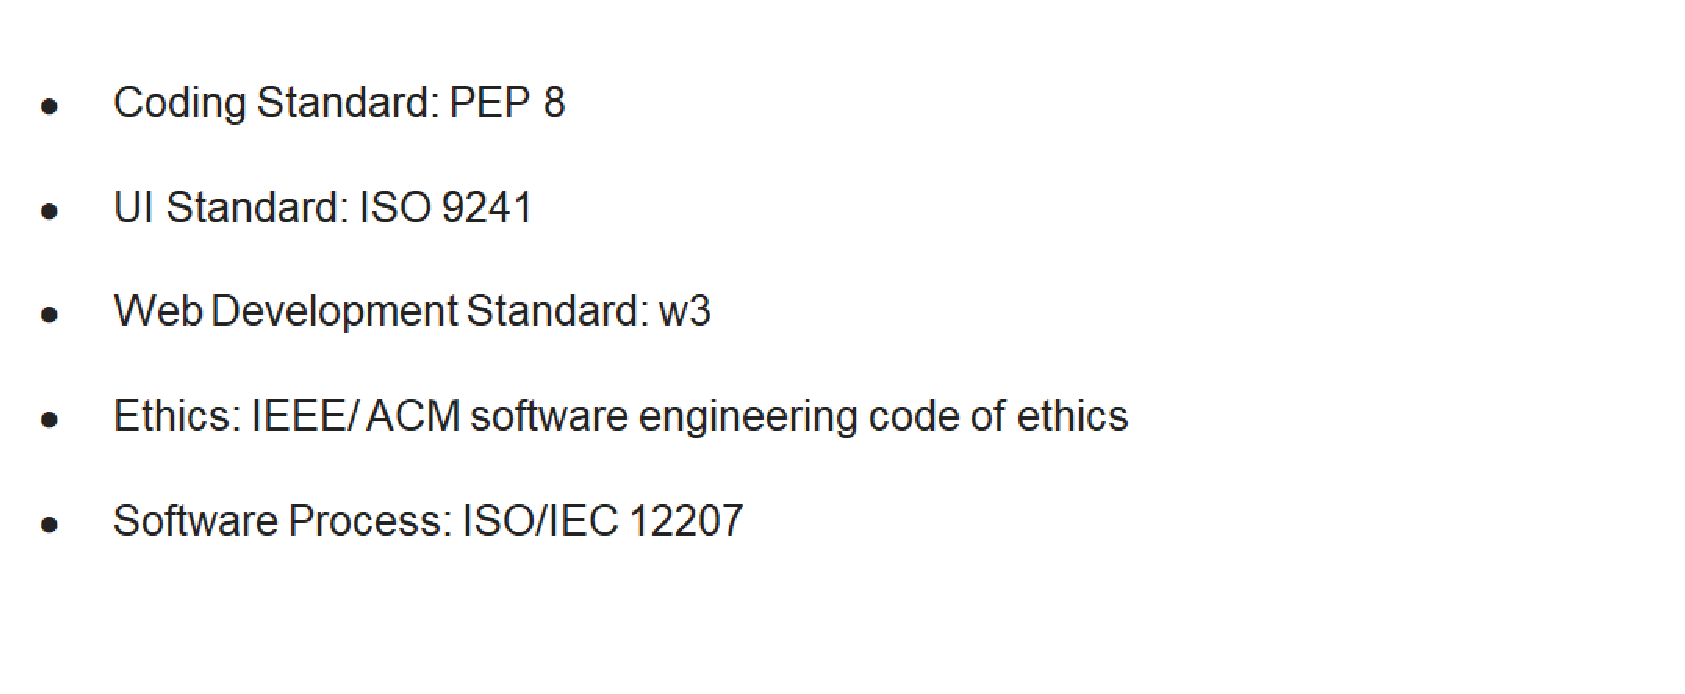
\includegraphics[width=\textwidth]{standard.eps}
 
\begin{description}[font=$\bullet$~\normalfont\scshape\color{red!50!black}]

\item Coding Standard: PEP 8
\item UI Standard: ISO 9241
\item Web Development Standard: w3
\item Ethics: IEEE/ ACM software engineering code of ethics
\item Software Process: ISO/IEC 12207

%\item [Coding Standard: ] PEP 8
%\item [UI Standard: ] ISO 9241
%\item [Web Development Standard: ] w3
%\item [Ethics: ] IEEE/ ACM software engineering code of ethics
%\item [Software Process: ] ISO/IEC 12207
\end{description}
 
As we are working on python so we have used PEP 8. ISO 9241 which is an international standard for UI, many country take it as their national standard so we took it as our UI standard. For web development we followed w3 because it is well organized platform. In ethical standard we have followed IEEE/ACM as they maintain professional standard. And lastly in software process we followed ISO/IEC 12207 because it gives us a common framework on the process of software life cycle.

\section{Challenges}

We have developed our tool using python for machine learning algorithm python flask package as API for parsing data from the input field to the machine learning algorithm. And we have also used HTML and CSS for the front end of the tool. The developed system is little bit different from other systems available right now. The system can't be run like other web tools just by coping the data on the server and hitting the web route. To run this system Linux server is must which allows installation of 3rd party application on which the system relies on. Linux server allows root level bash scripting which enables us to install dependencies for the system. But the issue with Linux server is it's not chip. But our university has helped us by providing us with a Linux server which helped us overcome the financial issue on buying a Linux server.\\
To be a capstone project every project needs to solve some complex issue. We think previous problem was one of them. And we have solved that problem with the help of our university authority. So this satisfies the condition of a project being a capstone project.

\section{Summary}

In this chapter we know about our projects social, biological, machine learning, economic, ethical impacts and constraint of our project and standards which we are following.


